\begin{figure}[hbtp]
  \centering
  \subfigure{
    \label{fig:leidenopt-modularity--all}
    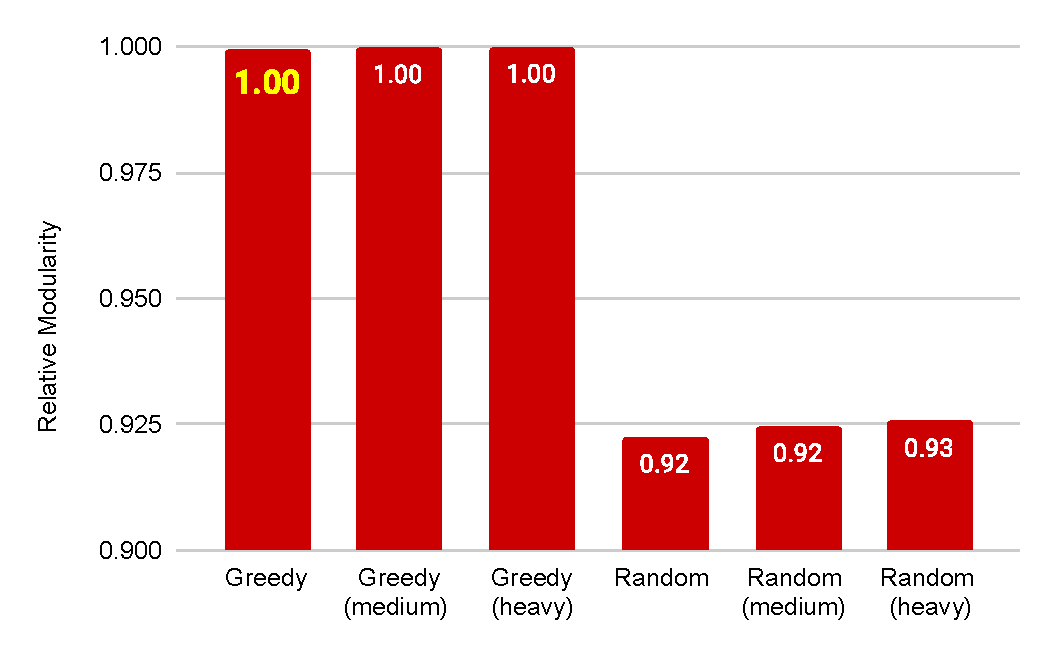
\includegraphics[width=0.98\linewidth]{out/leidenopt-modularity.pdf}
  } \\[-2ex]
  \caption{Average relative modularity for the \textit{greedy} and \textit{random} approaches (including \textit{medium} and \textit{heavy} variants) of parallel Leiden algorithm for all graphs in the dataset.}
  \label{fig:leidenopt-modularity}
\end{figure}
